\documentclass[12pt,a4paper]{article}
\usepackage{lmodern}

\usepackage{scalerel}
\usepackage{bbm}
\usepackage{enumitem}
\usepackage{placeins}
\usepackage{amssymb,amsmath}
\usepackage{ifxetex,ifluatex}
\usepackage{fixltx2e} % provides \textsubscript
\ifnum 0\ifxetex 1\fi\ifluatex 1\fi=0 % if pdftex
  \usepackage[T1]{fontenc}
  \usepackage[utf8]{inputenc}
\else % if luatex or xelatex
  \ifxetex
    \usepackage{mathspec}
    \usepackage{xltxtra,xunicode}
  \else
    \usepackage{fontspec}
  \fi
  \defaultfontfeatures{Mapping=tex-text,Scale=MatchLowercase}
  \newcommand{\euro}{€}
\fi
% use upquote if available, for straight quotes in verbatim environments
\IfFileExists{upquote.sty}{\usepackage{upquote}}{}
% use microtype if available
\IfFileExists{microtype.sty}{%
\usepackage{microtype}
\UseMicrotypeSet[protrusion]{basicmath} % disable protrusion for tt fonts
}{}
\usepackage[lmargin = 2cm, rmargin = 2cm, tmargin = 2cm, bmargin = 2.5cm]{geometry}


% Figure Placement:
\usepackage{float}
\let\origfigure\figure
\let\endorigfigure\endfigure
\renewenvironment{figure}[1][2] {
    \expandafter\origfigure\expandafter[H]
} {
    \endorigfigure
}

%%%% Jens %%%%
\usepackage{titlesec}
\DeclareMathOperator*{\argmax}{arg\,max}
\DeclareMathOperator*{\argmin}{arg\,min}
\renewcommand{\vec}{\operatorname{vec}}
\newcommand{\tr}{\operatorname{tr}}
\newcommand{\Var}{\operatorname{Var}} % Variance
\newcommand{\MSE}{\operatorname{MSE}} % Variance
\newcommand{\VAR}{\operatorname{VAR}} % Vector autoregression
\newcommand{\Lag}{\operatorname{L}} % Lag operator
\newcommand{\Cov}{\operatorname{Cov}}
\newcommand{\diag}{\operatorname{diag}}
\newcommand{\adj}{\operatorname{adj}}
\newcommand{\loglik}{\operatorname{ll}}

\usepackage{centernot}
\usepackage{mathtools}

\allowdisplaybreaks

\titleformat{\section}
{\normalfont\large\bfseries}{\thesection}{1em}{}

\newcommand{\tmpsection}[1]{}
\let\tmpsection=\section
\renewcommand{\section}[1]{\tmpsection{\underline{#1}} }





%% citation setup
\usepackage{csquotes}

\usepackage[backend=biber, maxbibnames = 99, style = apa]{biblatex}
\setlength\bibitemsep{1.5\itemsep}
\addbibresource{R_packages.bib}
\usepackage{color}
\usepackage{fancyvrb}
\newcommand{\VerbBar}{|}
\newcommand{\VERB}{\Verb[commandchars=\\\{\}]}
\DefineVerbatimEnvironment{Highlighting}{Verbatim}{commandchars=\\\{\}}
% Add ',fontsize=\small' for more characters per line
\usepackage{framed}
\definecolor{shadecolor}{RGB}{248,248,248}
\newenvironment{Shaded}{\begin{snugshade}}{\end{snugshade}}
\newcommand{\AlertTok}[1]{\textcolor[rgb]{0.94,0.16,0.16}{#1}}
\newcommand{\AnnotationTok}[1]{\textcolor[rgb]{0.56,0.35,0.01}{\textbf{\textit{#1}}}}
\newcommand{\AttributeTok}[1]{\textcolor[rgb]{0.77,0.63,0.00}{#1}}
\newcommand{\BaseNTok}[1]{\textcolor[rgb]{0.00,0.00,0.81}{#1}}
\newcommand{\BuiltInTok}[1]{#1}
\newcommand{\CharTok}[1]{\textcolor[rgb]{0.31,0.60,0.02}{#1}}
\newcommand{\CommentTok}[1]{\textcolor[rgb]{0.56,0.35,0.01}{\textit{#1}}}
\newcommand{\CommentVarTok}[1]{\textcolor[rgb]{0.56,0.35,0.01}{\textbf{\textit{#1}}}}
\newcommand{\ConstantTok}[1]{\textcolor[rgb]{0.00,0.00,0.00}{#1}}
\newcommand{\ControlFlowTok}[1]{\textcolor[rgb]{0.13,0.29,0.53}{\textbf{#1}}}
\newcommand{\DataTypeTok}[1]{\textcolor[rgb]{0.13,0.29,0.53}{#1}}
\newcommand{\DecValTok}[1]{\textcolor[rgb]{0.00,0.00,0.81}{#1}}
\newcommand{\DocumentationTok}[1]{\textcolor[rgb]{0.56,0.35,0.01}{\textbf{\textit{#1}}}}
\newcommand{\ErrorTok}[1]{\textcolor[rgb]{0.64,0.00,0.00}{\textbf{#1}}}
\newcommand{\ExtensionTok}[1]{#1}
\newcommand{\FloatTok}[1]{\textcolor[rgb]{0.00,0.00,0.81}{#1}}
\newcommand{\FunctionTok}[1]{\textcolor[rgb]{0.00,0.00,0.00}{#1}}
\newcommand{\ImportTok}[1]{#1}
\newcommand{\InformationTok}[1]{\textcolor[rgb]{0.56,0.35,0.01}{\textbf{\textit{#1}}}}
\newcommand{\KeywordTok}[1]{\textcolor[rgb]{0.13,0.29,0.53}{\textbf{#1}}}
\newcommand{\NormalTok}[1]{#1}
\newcommand{\OperatorTok}[1]{\textcolor[rgb]{0.81,0.36,0.00}{\textbf{#1}}}
\newcommand{\OtherTok}[1]{\textcolor[rgb]{0.56,0.35,0.01}{#1}}
\newcommand{\PreprocessorTok}[1]{\textcolor[rgb]{0.56,0.35,0.01}{\textit{#1}}}
\newcommand{\RegionMarkerTok}[1]{#1}
\newcommand{\SpecialCharTok}[1]{\textcolor[rgb]{0.00,0.00,0.00}{#1}}
\newcommand{\SpecialStringTok}[1]{\textcolor[rgb]{0.31,0.60,0.02}{#1}}
\newcommand{\StringTok}[1]{\textcolor[rgb]{0.31,0.60,0.02}{#1}}
\newcommand{\VariableTok}[1]{\textcolor[rgb]{0.00,0.00,0.00}{#1}}
\newcommand{\VerbatimStringTok}[1]{\textcolor[rgb]{0.31,0.60,0.02}{#1}}
\newcommand{\WarningTok}[1]{\textcolor[rgb]{0.56,0.35,0.01}{\textbf{\textit{#1}}}}
\usepackage{graphicx}
\makeatletter
\def\maxwidth{\ifdim\Gin@nat@width>\linewidth\linewidth\else\Gin@nat@width\fi}
\def\maxheight{\ifdim\Gin@nat@height>\textheight\textheight\else\Gin@nat@height\fi}
\makeatother
% Scale images if necessary, so that they will not overflow the page
% margins by default, and it is still possible to overwrite the defaults
% using explicit options in \includegraphics[width, height, ...]{}
\setkeys{Gin}{width=\maxwidth,height=\maxheight,keepaspectratio}
\ifxetex
  \usepackage[setpagesize=false, % page size defined by xetex
              unicode=false, % unicode breaks when used with xetex
              xetex]{hyperref}
\else
  \usepackage[unicode=true, linktocpage = TRUE]{hyperref}
\fi
\hypersetup{breaklinks=true,
            bookmarks=true,
            pdfauthor={Dr.~Yannick Hoga},
            pdftitle={Multivariate Time Series Analysis},
            colorlinks=true,
            citecolor=black,
            urlcolor=black,
            linkcolor=black,
            pdfborder={0 0 0}}
\urlstyle{same}  % don't use monospace font for urls
\setlength{\parindent}{0pt}
\setlength{\parskip}{6pt plus 2pt minus 1pt}
\setlength{\emergencystretch}{3em}  % prevent overfull lines
\setcounter{secnumdepth}{5}

%%% Use protect on footnotes to avoid problems with footnotes in titles
\let\rmarkdownfootnote\footnote%
\def\footnote{\protect\rmarkdownfootnote}

%%% Change title format to be more compact
\usepackage{titling}

% Create subtitle command for use in maketitle
\newcommand{\subtitle}[1]{
  \posttitle{
    \begin{center}\large#1\end{center}
    }
}

\setlength{\droptitle}{-2em}
  \title{Multivariate Time Series Analysis}
  \pretitle{\vspace{\droptitle}\centering\huge}
  \posttitle{\par}
\subtitle{Solution Exercise Sheet 9}
  \author{Dr.~Yannick Hoga}
  \preauthor{\centering\large\emph}
  \postauthor{\par}
  \date{}
  \predate{}\postdate{}


%% linespread settings

\usepackage{setspace}

\onehalfspacing


% Language Setup

\usepackage{ifthen}
\usepackage{iflang}
\usepackage[super]{nth}
\usepackage[ngerman, english]{babel}

%Acronyms
\usepackage[printonlyused, withpage, nohyperlinks]{acronym}
\usepackage{changepage}

% Multicols for the Title page
\usepackage{multicol}


% foot


\begin{document}

\selectlanguage{english}

%%%%%%%%%%%%%% Jens %%%%%
\numberwithin{equation}{section}




\restoregeometry


%%% Header 

\begin{minipage}{0.6\textwidth}
University of Duisburg-Essen\\
Faculty of Business Administration and Economics\\
Chair of Econometrics\\
\end{minipage}

%\begin{minipage}{0.4\textwidth}
	\begin{flushright}
	\vspace{-3cm}
	\includegraphics*[width=5cm]{../Includes/duelogo_en.png}\\
	\vspace{.125cm}
	\end{flushright}
%\end{minipage}
%\vspace{.125cm}
\hspace{-0.005cm}Winter Term 2019/2020

\vspace{0.05cm}

\begin{center}
	\vspace{.25cm}
	Dr.~Yannick Hoga \hspace{.5cm} Thilo Reinschlüssel \\
	\vspace{.25cm}
	\textbf{\Large{Multivariate Time Series Analysis}}\\
	\vspace{.25cm}
	\textbf{\large{Solution Exercise Sheet 9}}\\
	\vspace{.125cm}
\end{center}




% body from markdown

\hypertarget{exercise-1-granger-causality-theory}{%
\section{Exercise 1: Granger Causality --
Theory}\label{exercise-1-granger-causality-theory}}

Let \(z_t = (x_t, y_t)^{'}\) be a stationary time series with two
dimensions. Define the forecast errar as the univariare series
\(e_T (h) = y_{T +h} - y_T (h)\) with
\(y_T (h) = \mathbb{E} \left( y_{T + h} | \Omega_T \right)\). The
information set \(\Omega_T\) contains all relevant variables available
whereas
\(\Omega^{\setminus x}_{T} = \Omega_T \setminus \left\{ x_t\right\}_{t = 0}^{T}\)
omits the variable \(x\) entirely. (This setting is the univariate
equivalent to definition 6.1 on Slide 6-4.)

\begin{itemize}
  \item[a)] Prove that $\mathbb{E} \left( e_T(h) | \Omega_{T}^{\setminus x} \right) = 0$.
\end{itemize}

\emph{Solution:}

\begin{align*}
  z_t & = \begin{pmatrix} x_t \\ y_t \end{pmatrix}\\
  \\
  \mathbb{E} \left( e_T (h) | \Omega_{T}^{\setminus x} \right) & = \mathbb{E} \left( y_{T + h} - \mathbb{E} \left( y_{T +h} | \Omega_T \right) | \ \Omega_{T}^{\setminus x} \right)\\
  & \overset{\text{LIE}}{=} \mathbb{E} \left( \mathbb{E} \left( y_{T +h} - y_{T + h}| \Omega_T \right) | \Omega_{T}^{\setminus x} \right)\\
  & \text{since } \Omega_{T}^{\setminus x} \subseteq \Omega_{T}  \\
  & \text{LIE = Law of Iterated Expectations}\\
  & = 0\\
\end{align*}

\begin{itemize}
  \item[b)] Prove that $\Var \left(e_t (h)| \Omega_T \right) \leq \Var \left(e_t (h)| \Omega_T^{\setminus x} \right)$
\end{itemize}

\emph{Solution:}

2 Theorems necessary for the proof:

\(1.\) Conditional Jensen's Inequality

\(g(\cdot ): \mathbb{R}^{m} \rightarrow \mathbb{R}\) is convex (like
\(\chi^2\)), then for any random vectors (y,x) for which
\(\mathbb{E} (||y||) < \infty\) and \(\mathbb{E} (|| g(y)||)< \infty\),
\(g \left( \mathbb{E} (y|x) \right) \leq \mathbb{E} \left( (g(y)|x) \right)\).
It is the other way around for concave functions.

\(2.\) Conditioning Theorem

If \(\mathbb{E}(|y|) < \infty\), then
\(\mathbb{E}(g(x) y | x) = g(x) \cdot \mathbb{E}(y|x)\). If in addition
\(\mathbb{E} (|g(x) y|) < \infty\), then
\(\mathbb{E} (g(x) y) = \mathbb{E} (g(x) \mathbb{E} (y|x))\).

Back to Granger:

\(e_T (h) = y_{T +h} - y_T (h)\) is a scalar. We know that
\(\mathbb{E} \left( e_T (h) | \Omega_T^{ \setminus x} \right) = 0\),
\(\mathbb{E} \left( e_T (h) | \Omega_T \right) = 0\) and
\(\Var(e_T (h)) < \infty\) since \(y_t\) is a weakly stationary (w.s.)
process. Furthermore, w.s. implies that
\(\mathbb{E} (y_t) < \infty, \mathbb{E} (y_t^2) < \infty\).

From Jensen's Inequality it follows:

\begin{align*}
  \left[ \mathbb{E} \left( y_{T + h} | \Omega_{T}^{\setminus x } \right) \right]^2 & \overset{\text{LIE}}{=} \left[ \mathbb{E} \left[ \mathbb{E} \left( y_{T + h} | \Omega_{T} \right) | \Omega_T^{\setminus x} \right] \right]^2 \\
  & \leq \mathbb{E} \left[ \left[ \mathbb{E} (y_{t +h} | \Omega_T)\right]^2 | \Omega_{t}^{\setminus x} \right]
\end{align*}

Taking conditional expectations:

\begin{align}
  \mathbb{E} \left[ \left( \mathbb{E}\left[ y_{T + h | \Omega_{T}^{\setminus x}} \right]  \right)^2 \right] \leq \mathbb{E} \left( \left[ \mathbb{E} \left( y_{T +h} | \Omega_T \right) \right]^2 \right) \label{eq:1}
\end{align}

This extends to:

\begin{align}
  \left[ \mathbb{E} (y_{T + h}) \right]^2 & \leq \mathbb{E}  \left( \left[ \mathbb{E} \left( y_{T + h} | \Omega_T^{\setminus x} \right) \right]^2 \right) \label{eq:2}\\
  \text{Since} \; \; \mathbb{E} (y_{T + h}) & = \mathbb{E} \left[ \mathbb{E} \left( y_{T +h} | \Omega_{T}^{\setminus x}\right) \right] \nonumber \\
  & = \mathbb{E} \left[ \mathbb{E} \left( y_{T +h} | \Omega_{T}\right) \right] \nonumber
\end{align}

the inequations \eqref{eq:1} and \eqref{eq:2} imply similar ranking for
the variances:

\begin{align*}
0 & \leq \Var \left( \mathbb{E} \left[ y_{T + h} | \Omega_{T}^{\setminus x} \right] \right) \leq \Var \left( \mathbb{E} \left[ y_{T + h} | \Omega_{T} \right] \right) \\
  & \text{since} \Var(z) = \mathbb{E} (z^2) - \left[ \mathbb{E} (z) \right]^2
\end{align*}

Consider the decomposition below:

\begin{align*}
  y_{T + h} - \mu & = \underbrace{ y_{T + h} - \mathbb{E} \left( y_{T + h} | \Omega \right)}_{e_T (h)| \Omega} + \underbrace{\mathbb{E} \left( y_{T + h} | \Omega \right) - \mu}_{u_T (h) | \Omega} 
\end{align*}

Remember that:

\begin{align*}
  \mathbb{E} [e_T (h)| \Omega] & = 0 \quad \text{for} \quad \Omega = \left\{ \Omega_T, \Omega_T^{\setminus x} \right\} \\
  \text{and } \mathbb{E} [e_T (h) * u_T (h)] & = 0 \Rightarrow \Cov(e_T (h), u_T (h)) = 0
\end{align*}

Thus:

\begin{align*}
  \Var \left( y_{T + h} - \mu | \Omega \right) & = \Var \left( e_T (h) + u_T (h) | \Omega \right) \\
  & = \Var \left( e_T (h)  | \Omega \right) +  \Var \left( u_T (h) | \Omega \right)
\end{align*}

Since \(\mu\) is a constant and \(y_{T + h}\) does not depend on
\(\Omega\):

\begin{align*}
  \Var\left(y_{T + h} - \mu | \Omega \right) & = \Var\left( y_{T + h}\right) \\
  \Var\left(u_{T} (h) | \Omega \right) & = \Var\left( \mathbb{E} [ y_{T + h} | \Omega ]\right) \\
  \Var\left(  y_{T + h} \right) & = \Var\left(  e_{T} h  | \Omega \right) + \Var\left( \mathbb{E} [ y_{T + h} | \Omega ]\right)
\end{align*}

We have already shown that

\begin{align*}
\Var \left( \mathbb{E}(y_{T + h} | \Omega_T) \right) \geq \Var \left( \mathbb{E} \left(y_{T +h} | \Omega_{T}^{\setminus x} \right) \right)
\end{align*}

and we know that \(\Var(y_{T +h}) = \sigma^2\) is constant. This
implies:

\begin{align*}
\Var\left(e_T (h) | \Omega_T \right) \leq \Var \left( e_T (h) | \Omega_T^{\setminus x} \right) \qquad _{\square}
\end{align*}

\hypertarget{exercise-2-granger-causality-and-irfs-in-data}{%
\section{Exercise 2: Granger Causality and IRFs in
Data}\label{exercise-2-granger-causality-and-irfs-in-data}}

We return to the dataset \texttt{fx\_series.Rda} and examine Granger
(Non)-Causality and the Impulse Response Functions (IRFs). Remember that
this dataset contains two time series of exchange rates.

\begin{itemize}
  \item[a)] Do you find any Granger Causality in a $\VAR(1)$ model? Which zero restrictions are implied for the coefficient matrix $\phi_1$?
\end{itemize}

\emph{Solution:}

\begin{Shaded}
\begin{Highlighting}[]
\CommentTok{# VAR(1) with intercept, no trends}
\NormalTok{var1.fit <-}\StringTok{ }\KeywordTok{VAR}\NormalTok{(fx_series, }\DataTypeTok{p =} \DecValTok{1}\NormalTok{, }\DataTypeTok{type =} \StringTok{"const"}\NormalTok{) }
\CommentTok{# there is conditional heteroscedasticity in the data, }
\CommentTok{#that's why employing a HC VCOV matric helps}
\KeywordTok{causality}\NormalTok{(}\DataTypeTok{x =}\NormalTok{ var1.fit, }\DataTypeTok{cause =} \StringTok{"lr.Eu"}\NormalTok{, }\DataTypeTok{vcov. =} \KeywordTok{vcovHC}\NormalTok{(var1.fit)) }
\end{Highlighting}
\end{Shaded}

\begin{verbatim}
## $Granger
## 
##  Granger causality H0: lr.Eu do not Granger-cause lr.Ja
## 
## data:  VAR object var1.fit
## F-Test = 0.00011986, df1 = 1, df2 = 10034, p-value = 0.9913
## 
## 
## $Instant
## 
##  H0: No instantaneous causality between: lr.Eu and lr.Ja
## 
## data:  VAR object var1.fit
## Chi-squared = 370.25, df = 1, p-value < 2.2e-16
\end{verbatim}

\begin{Shaded}
\begin{Highlighting}[]
\KeywordTok{causality}\NormalTok{(}\DataTypeTok{x =}\NormalTok{ var1.fit, }\DataTypeTok{cause =} \StringTok{"lr.Ja"}\NormalTok{, }\DataTypeTok{vcov. =} \KeywordTok{vcovHC}\NormalTok{(var1.fit))}
\end{Highlighting}
\end{Shaded}

\begin{verbatim}
## $Granger
## 
##  Granger causality H0: lr.Ja do not Granger-cause lr.Eu
## 
## data:  VAR object var1.fit
## F-Test = 2.9687, df1 = 1, df2 = 10034, p-value = 0.08492
## 
## 
## $Instant
## 
##  H0: No instantaneous causality between: lr.Ja and lr.Eu
## 
## data:  VAR object var1.fit
## Chi-squared = 370.25, df = 1, p-value < 2.2e-16
\end{verbatim}

The \(H_0\) of Granger \emph{Non}-Causality is never rejected.

\begin{align*}
  z_t = \phi_0 + \begin{pmatrix} \ast & 0 \\ 0 & \ast \end{pmatrix} z_{t - 1} + a_t
\end{align*}

\begin{itemize}
  \item[b)] Is there evidence for instantaneous causality? Whar are the implications regarding $\Sigma_a$?
\end{itemize}

\emph{Solution:}

Yes, the \(H_0\) is rejected (in the test from a) ).There is evidence
for instantaneous Causality meaning that \(\Sigma_a\) has non-zero
entries of the main diagonal.

\begin{align*}
  \Sigma_a = \begin{pmatrix} \ast & \sigma_{12}  \\ \sigma_{12} & \ast \end{pmatrix} , \quad \sigma_{12} \neq 0 
\end{align*}

\begin{itemize}
  \item[c)] Before you plot the IRFs, make a guess about their appearance based on Granger Causality. Then compute the IRFs (do \emph{not} use orthogonal innovations!) for five periods and comment.
\end{itemize}

\emph{Solution:}

\begin{Shaded}
\begin{Highlighting}[]
\NormalTok{irf1 <-}\StringTok{ }\KeywordTok{irf}\NormalTok{(}\DataTypeTok{x =}\NormalTok{ var1.fit, }\DataTypeTok{ortho =} \OtherTok{FALSE}\NormalTok{, }\DataTypeTok{n.ahead =} \DecValTok{5}\NormalTok{)}
\CommentTok{# plot IRFs of shock on first exchange rate}
\KeywordTok{plot}\NormalTok{(}\DataTypeTok{x =} \DecValTok{0}\OperatorTok{:}\DecValTok{5}\NormalTok{, irf1}\OperatorTok{$}\NormalTok{irf}\OperatorTok{$}\NormalTok{lr.Eu[,}\DecValTok{1}\NormalTok{], }\DataTypeTok{ylim =} \KeywordTok{c}\NormalTok{(}\DecValTok{0}\NormalTok{,}\DecValTok{1}\NormalTok{), }\DataTypeTok{type =} \StringTok{"l"}\NormalTok{, }\DataTypeTok{col =} \StringTok{"red"}
\NormalTok{     , }\DataTypeTok{main =} \StringTok{"IRF of shock on lr.Eu"}\NormalTok{)}
\KeywordTok{points}\NormalTok{(}\DataTypeTok{x =} \DecValTok{0}\OperatorTok{:}\DecValTok{5}\NormalTok{, }\DataTypeTok{y =}\NormalTok{ irf1}\OperatorTok{$}\NormalTok{irf}\OperatorTok{$}\NormalTok{lr.Eu[,}\DecValTok{2}\NormalTok{], }\DataTypeTok{type =} \StringTok{"l"}\NormalTok{, }\DataTypeTok{col =} \StringTok{"blue"}\NormalTok{)}
\KeywordTok{legend}\NormalTok{(}\StringTok{"topright"}\NormalTok{, }\DataTypeTok{legend =} \KeywordTok{c}\NormalTok{(}\StringTok{"lr.Eu"}\NormalTok{,}\StringTok{"lr.Ja"}\NormalTok{), }\DataTypeTok{lwd =} \KeywordTok{c}\NormalTok{(}\DecValTok{2}\NormalTok{,}\DecValTok{2}\NormalTok{), }\DataTypeTok{col =} \KeywordTok{c}\NormalTok{(}\StringTok{"red"}\NormalTok{, }\StringTok{"blue"}\NormalTok{))}
\end{Highlighting}
\end{Shaded}

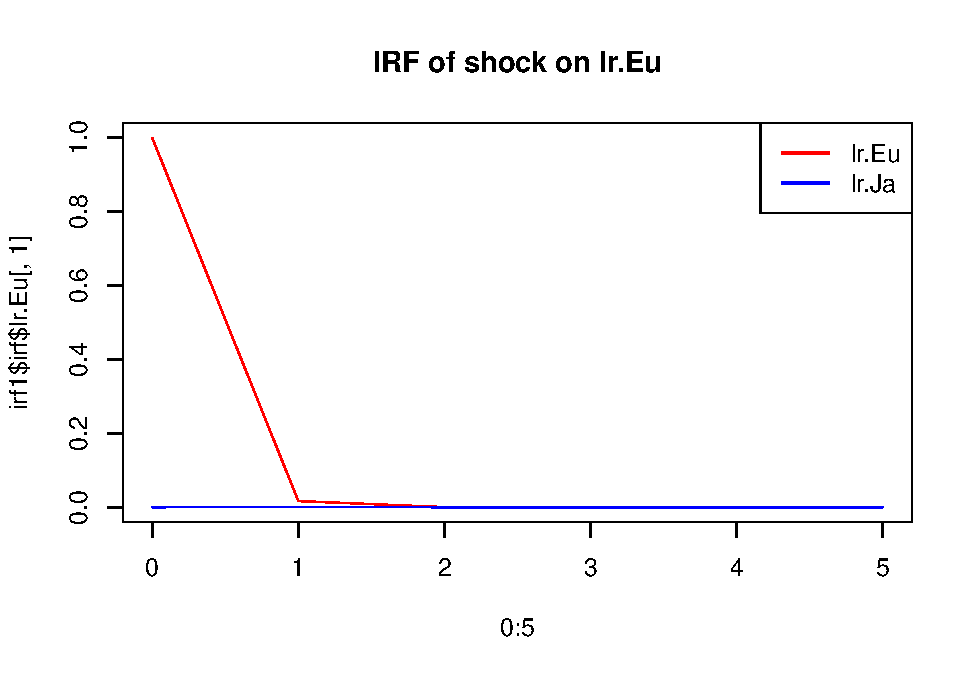
\includegraphics{solution_exercise_9_files/figure-latex/2_c-1.pdf}

\begin{Shaded}
\begin{Highlighting}[]
\CommentTok{# plot IRFs of shock on second exchange rate}
\KeywordTok{plot}\NormalTok{(}\DataTypeTok{x =} \DecValTok{0}\OperatorTok{:}\DecValTok{5}\NormalTok{, irf1}\OperatorTok{$}\NormalTok{irf}\OperatorTok{$}\NormalTok{lr.Ja[,}\DecValTok{1}\NormalTok{], }\DataTypeTok{ylim =} \KeywordTok{c}\NormalTok{(}\DecValTok{0}\NormalTok{,}\DecValTok{1}\NormalTok{), }\DataTypeTok{type =} \StringTok{"l"}\NormalTok{, }\DataTypeTok{col =} \StringTok{"red"}
\NormalTok{     , }\DataTypeTok{main =} \StringTok{"IRF of shock on lr.Ja"}\NormalTok{)}
\KeywordTok{points}\NormalTok{(}\DataTypeTok{x =} \DecValTok{0}\OperatorTok{:}\DecValTok{5}\NormalTok{, }\DataTypeTok{y =}\NormalTok{ irf1}\OperatorTok{$}\NormalTok{irf}\OperatorTok{$}\NormalTok{lr.Ja[,}\DecValTok{2}\NormalTok{], }\DataTypeTok{type =} \StringTok{"l"}\NormalTok{, }\DataTypeTok{col =} \StringTok{"blue"}\NormalTok{)}
\KeywordTok{legend}\NormalTok{(}\StringTok{"topright"}\NormalTok{, }\DataTypeTok{legend =} \KeywordTok{c}\NormalTok{(}\StringTok{"lr.Eu"}\NormalTok{,}\StringTok{"lr.Ja"}\NormalTok{), }\DataTypeTok{lwd =} \KeywordTok{c}\NormalTok{(}\DecValTok{2}\NormalTok{,}\DecValTok{2}\NormalTok{), }\DataTypeTok{col =} \KeywordTok{c}\NormalTok{(}\StringTok{"red"}\NormalTok{, }\StringTok{"blue"}\NormalTok{))}
\end{Highlighting}
\end{Shaded}

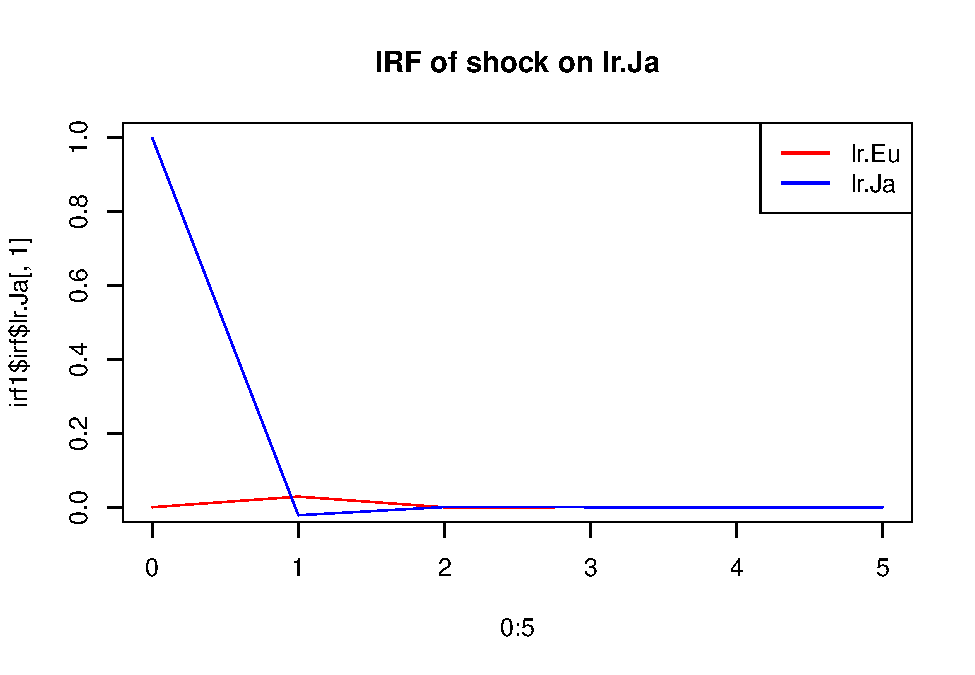
\includegraphics{solution_exercise_9_files/figure-latex/2_c-2.pdf}

\begin{Shaded}
\begin{Highlighting}[]
\NormalTok{irf1}\OperatorTok{$}\NormalTok{irf}\OperatorTok{$}\NormalTok{lr.Eu}
\end{Highlighting}
\end{Shaded}

\begin{verbatim}
##             lr.Eu         lr.Ja
## [1,] 1.000000e+00  0.000000e+00
## [2,] 1.659978e-02  2.009948e-04
## [3,] 2.813309e-04 -1.032811e-06
## [4,] 4.640339e-06  7.899758e-08
## [5,] 7.929965e-08 -7.845867e-10
## [6,] 1.293801e-09  3.299438e-11
\end{verbatim}

\begin{Shaded}
\begin{Highlighting}[]
\NormalTok{irf1}\OperatorTok{$}\NormalTok{irf}\OperatorTok{$}\NormalTok{lr.Ja}
\end{Highlighting}
\end{Shaded}

\begin{verbatim}
##              lr.Eu         lr.Ja
## [1,]  0.000000e+00  1.000000e+00
## [2,]  2.874839e-02 -2.173827e-02
## [3,] -1.477234e-04  4.783307e-04
## [4,]  1.129906e-05 -1.042778e-05
## [5,] -1.122198e-07  2.289529e-07
## [6,]  4.719202e-09 -4.999595e-09
\end{verbatim}

No evidence for Granger Causality between \(z_{1, t}\) and \(z_{2, t}\)

\(\Rightarrow a_{1,t}\) barely influences \(z_{2, t}\) if we control for
\(a_{2, t}\) and vice versa.

As expected, unit impulses on either \(a_{1, t} / a_{2, t}\) did not
affect \(z_{2, t}/ z_{1, t}\) by much. The impulse vanishes quickly.

\hypertarget{exercise-3-granger-non-causality-and-irfs}{%
\section{Exercise 3: Granger Non-Causality and
IRFs}\label{exercise-3-granger-non-causality-and-irfs}}

Consider a general three-dimensional \(\VAR(1)\) in which the first
variable \(z_{1, t}\) does not Granger cause the other variables. Show
that a shock \(a_{1,T}\) does not affect
\(\left\{ z_{2, t}\right\}_{t = T}^{\infty}\) and
\(\left\{ z_{3, t}\right\}_{t = T}^{\infty}\).

\emph{Solution:}

\begin{align*}
  z_t & = \phi_1 z_{t-1} + a_t \\
  \\
  \{z_{1, t}\} & \centernot{\rightarrow} \left\{ z_{2, \cdot}, z_{3, \cdot}\right\}\\
  \\
  \Rightarrow \phi_1 & = \begin{pmatrix} 
  \ast & \ast & \ast \\
  0 & \ast & \ast \\
  0 & \ast & \ast \\
  \end{pmatrix} =  \begin{pmatrix} 
  a & b & c \\
  0 & d & e \\
  0 & f & g \\
  \end{pmatrix}
\end{align*}

Take \(\theta_S\) from the causal representation:

\begin{align*}
  \dfrac{\partial z_{t,s}}{\partial a_t} & = \theta_s \\
  z_{t + s} & = \sum_{i = 0}^{t + s -1} \theta_i a_{t + s -i}
\end{align*}

Special case for \(\VAR(1)\):

\(\theta_s = \phi_1^{2}\) and \(\theta_0 = I_{3 \times 3}\) which
fulfills the restrictions trivially as \(\theta_1\) does.

\begin{align*}
\theta_2 & = \begin{pmatrix} 
  a & b & c \\
  0 & d & e \\
  0 & f & g \\
  \end{pmatrix} \begin{pmatrix} 
  a & b & c \\
  0 & d & e \\
  0 & f & g \\
  \end{pmatrix} \\
  & = 
  \begin{pmatrix} 
  \ast & \ast & \ast \\
  0 \cdot a + d \cdot 0 + e \cdot 0 & \ast & \ast \\
  0 \cdot a + f \cdot 0 + g \cdot 0 & \ast & \ast \\
  \end{pmatrix}\\
  & = 
  \begin{pmatrix} 
  \ast    & \ast & \ast \\
  0       & \ast & \ast \\
  0       & \ast & \ast \\
  \end{pmatrix}
\end{align*}

\(\Rightarrow \theta_i = \phi_1 \cdot \theta_{i -1}\) does always
fulfill the restirctions for \(i \geq 0\). Therefore \(a_{1,t}\) does
never influences \(z_{2, \cdot}\) or \(z_{3, \cdot}\).
\(\qquad _{\square}\)

\end{document}
